\documentclass[12pt,a4paper]{article}

\usepackage[a4paper,margin=1in]{geometry}
\usepackage{graphicx}
\graphicspath{{./}{Ex8/}}
\usepackage{booktabs}
\usepackage{amsmath,amssymb}
\usepackage{float}
\usepackage{hyperref}
\usepackage{xcolor}
\usepackage{listings}
\usepackage{enumitem}
\usepackage{fancyhdr}
\usepackage{longtable}

\hypersetup{colorlinks=true,linkcolor=blue,urlcolor=blue}

\pagestyle{fancy}
\fancyhf{}
\setlength{\headheight}{15pt}
\lhead{ICS1512}
\rhead{Machine Learning Algorithms Laboratory}
\cfoot{\thepage}

\begin{document}

\begin{tabular}{|p{4cm}|p{11cm}|}
\hline
Experiment No. & 8 \\ \hline
Experiment Title & Clustering Human Activity Recognition Data using K-Means, DBSCAN, and Hierarchical Clustering\footnote{\textbf{GitHub Repository: }\url{https://github.com/Naren-Kandasamy/Machine_Learning_Lab-3122247001036}}\\ \hline
Student Name & Naren Karthik Kandasamy \\ \hline
Register Number & 3122247001036 \\ \hline
Faculty & Dr. Poreddy Ajay Kumar Reddy \\ \hline
Submission Date & 19/09/2026 \\ \hline
\end{tabular}

\vspace{1em}

\section{Objective}
To implement, tune, and evaluate unsupervised clustering algorithms on high-dimensional sensory data from the Human Activity Recognition (HAR) benchmark:
\begin{itemize}[noitemsep]
    \item \textbf{Model A:} K-Means Clustering optimized via the Elbow Method and Silhouette Analysis.
    \item \textbf{Model B:} Density-Based Spatial Clustering of Applications with Noise (DBSCAN) exploring spatial radius ($\epsilon$) and density thresholds ($minPts$).
    \item \textbf{Model C:} Hierarchical Agglomerative Clustering (HAC) exploring diverse linkage criteria (Ward, Complete, Average, Single).
\end{itemize}

\section{Problem Statement}
In pervasive computing and wearable health monitoring, physical movements are logged across multi-channel inertial sensors (accelerometers, gyroscopes). The goal is to discover natural kinetic groupings in an unsupervised 561-dimensional feature space without utilizing ground-truth labels during training, and to evaluate cluster validity using both internal geometric metrics and external ground-truth activity alignment.

\section{Dataset Description}
The \textbf{Human Activity Recognition Using Smartphones} dataset captures waist-mounted inertial sensor measurements across 30 volunteer participants performing daily living routines.
\begin{longtable}{|p{5.5cm}|p{9.5cm}|}
\hline
\textbf{Property} & \textbf{Specification} \\ \hline
Dataset Source & UCI Machine Learning Repository \\ \hline
Sensors & 3-Axis Accelerometer and 3-Axis Gyroscope (50 Hz) \\ \hline
Sampling Window & 2.56-second sliding windows (128 readings, 50\% overlap) \\ \hline
Total Instances & 10,299 instances (7,352 train + 2,947 test) \\ \hline
Feature Dimensions & 561 time- and frequency-domain extracted metrics \\ \hline
Ground-Truth Activities (6) & WALKING, WALKING\_UPSTAIRS, WALKING\_DOWNSTAIRS, SITTING, STANDING, LAYING \\ \hline
\end{longtable}

\section{Exploratory Data Analysis}
Exploratory analysis examines the intrinsic geometric distribution of physical activity clusters projected onto the primary 2D principal component manifold.

\begin{figure}[H]
\centering
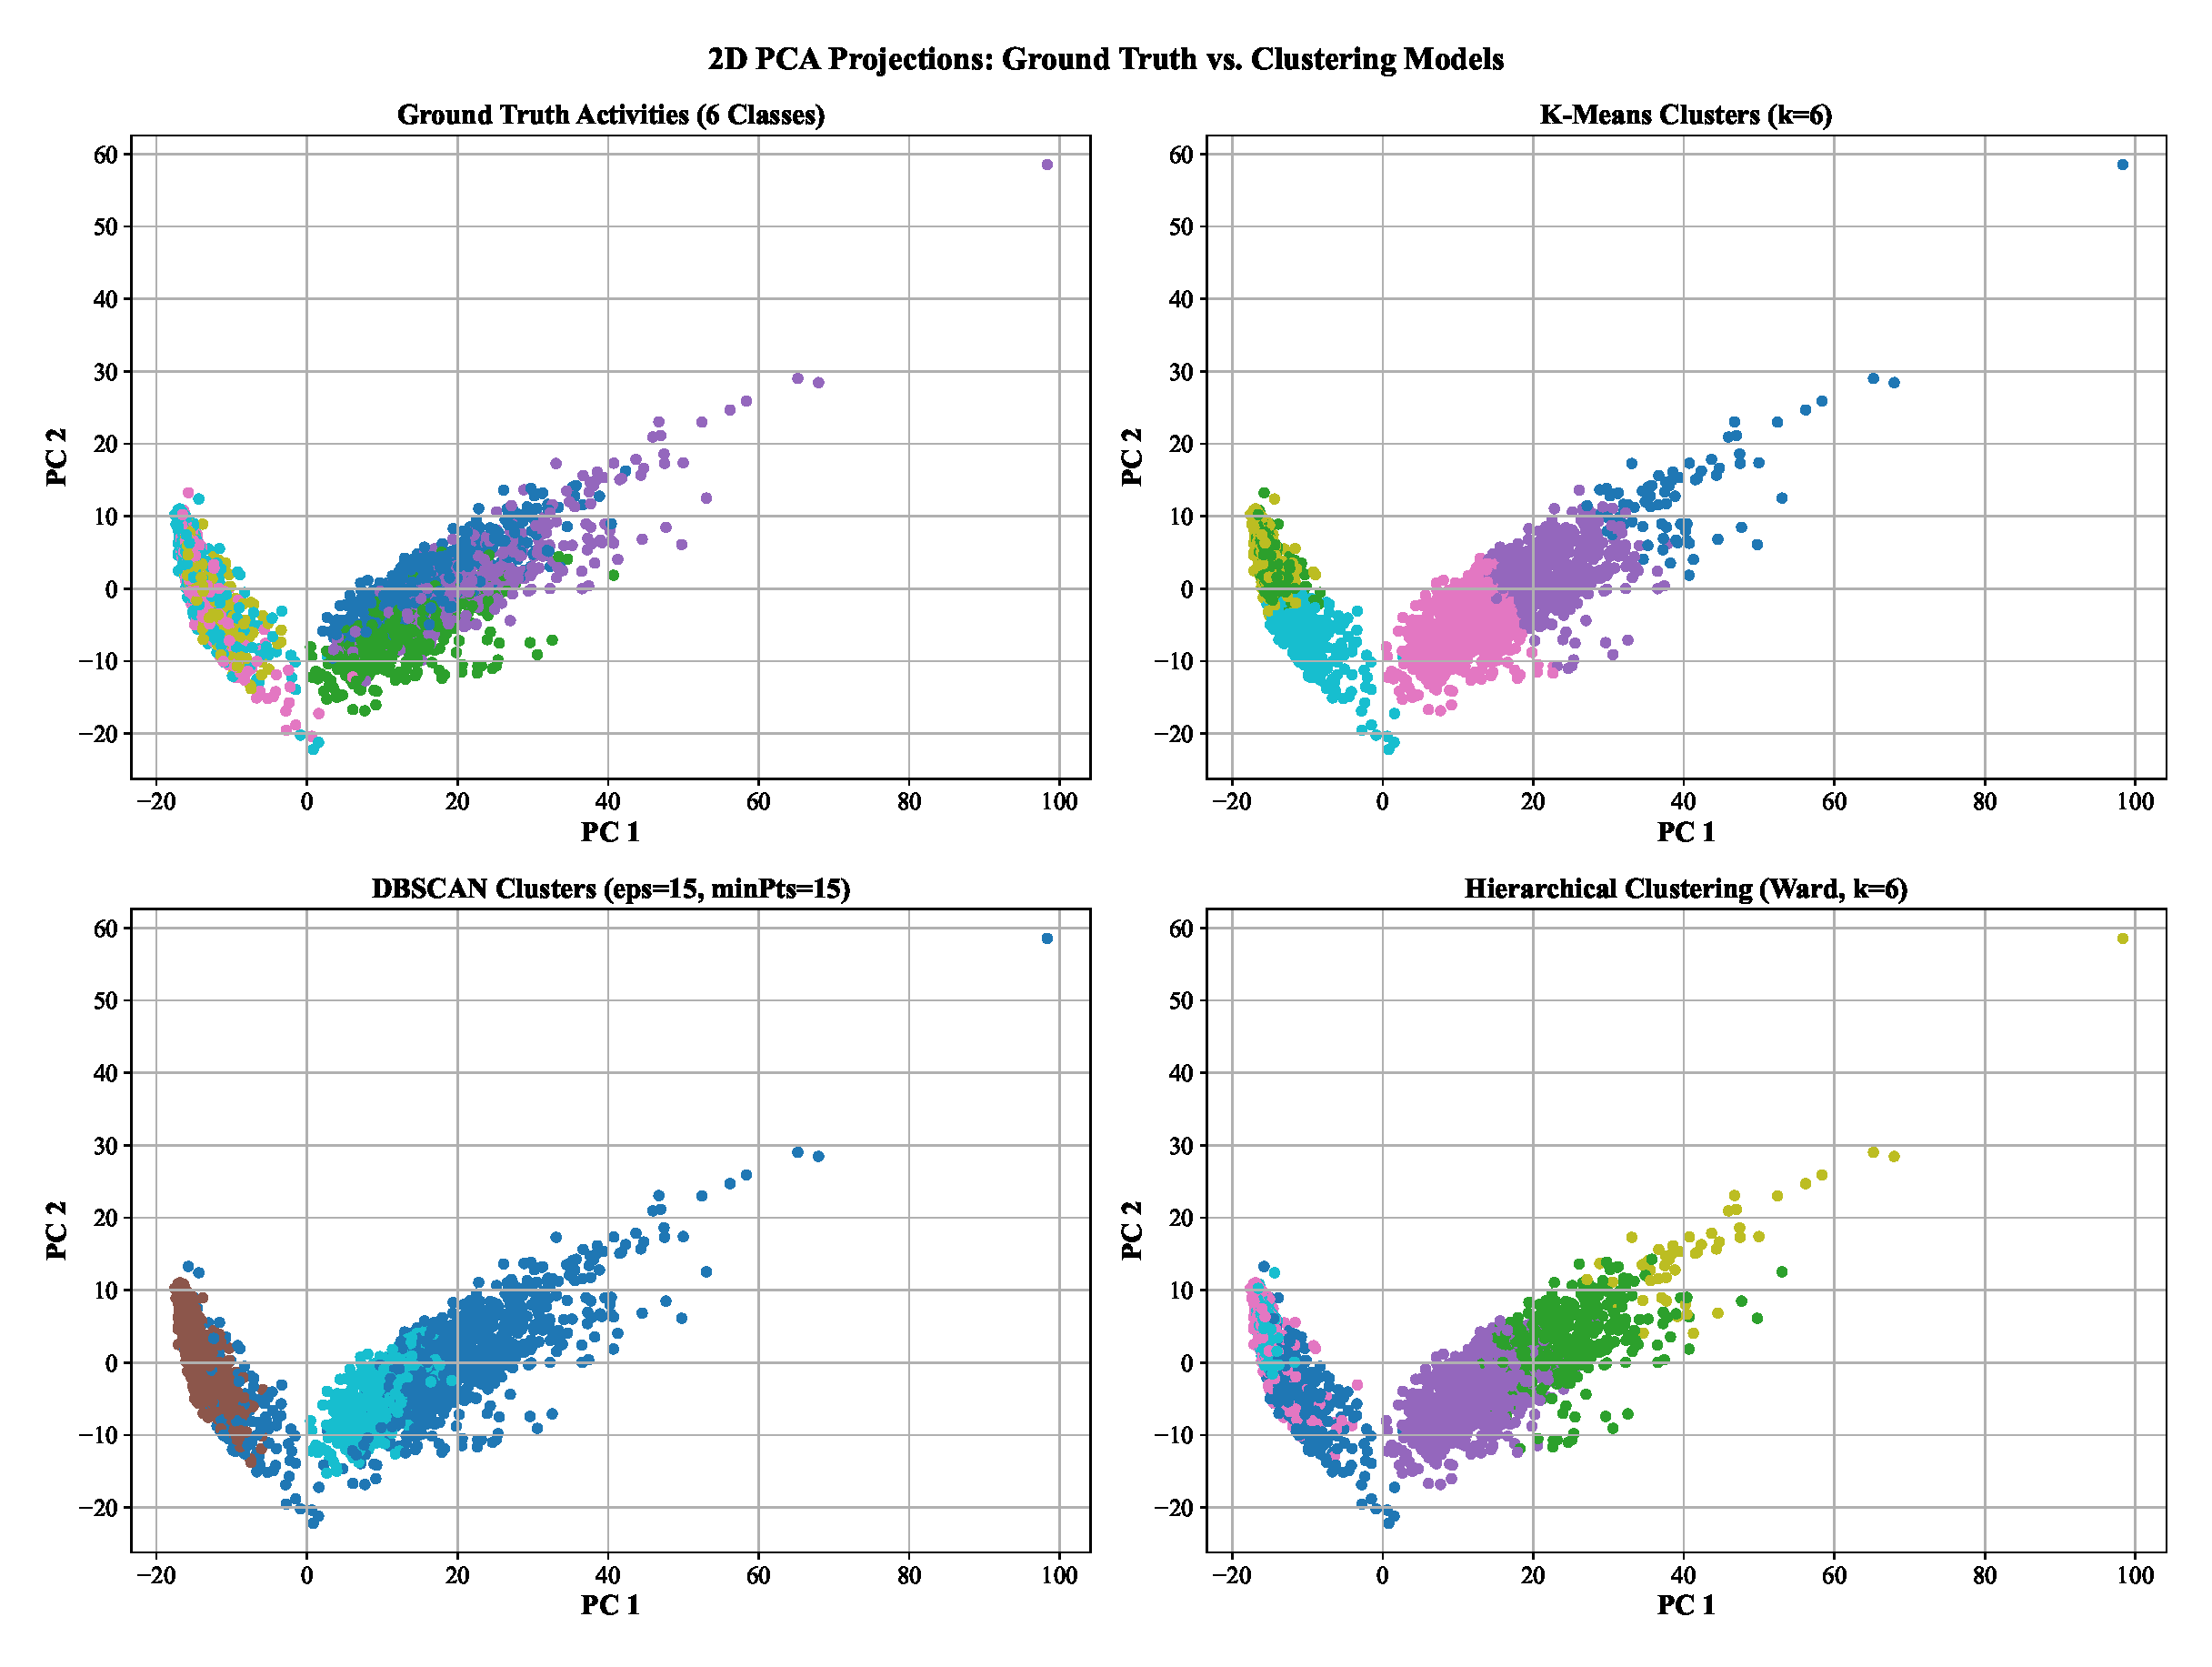
\includegraphics[width=0.88\linewidth]{Cluster_Scatter.eps}
\caption{2D PCA Visualizations: Ground Truth vs. K-Means, DBSCAN, and Hierarchical Clustering.}
\label{fig:eda_scatter}
\end{figure}

\textbf{Inference:}
The 2D projection reveals a pronounced macro-separation between dynamic kinetic states (walking, walking upstairs/downstairs) occupying the positive PC1 coordinate region, and static postural states (sitting, standing, laying) clustering in the negative PC1 domain. Overlaps between sitting and standing reflect shared static vertical sensor orientations.

\section{Data Preprocessing}
Sensor features are derived from Butterworth bandpass filtering (0.02--20 Hz) and Fast Fourier Transforms (FFT). To prevent high-variance inertial components from skewing Euclidean distances, features are standardized to zero mean and unit variance:
$$\mathbf{z} = \frac{\mathbf{x} - \mathbf{\mu}}{\mathbf{\sigma}}$$
Outlier transitions and boundary frames are preserved for DBSCAN noise isolation.

\section{Machine Learning Algorithm}
\subsection{K-Means Clustering}
Minimizes the Within-Cluster Sum of Squares (WCSS):
$$\text{WCSS} = \sum_{i=1}^k \sum_{\mathbf{x} \in S_i} \|\mathbf{x} - \mathbf{\mu}_i\|^2$$
\textbf{Advantages:} Efficient convergence ($O(n \cdot k \cdot t)$), scalable to large datasets. \textbf{Limitations:} Assumes spherical clusters of equal variance, sensitive to initial centroid placement.

\subsection{DBSCAN}
Classifies points as core points ($|N_\epsilon(\mathbf{p})| \ge minPts$), border points, or noise.
\textbf{Advantages:} Discovers arbitrary non-linear cluster geometries, robust to sensory outliers without pre-defining $k$. \textbf{Limitations:} Degrades in high-dimensional spaces due to distance concentration.

\subsection{Hierarchical Agglomerative Clustering (HAC)}
Builds a bottom-up hierarchical dendrogram using Ward's minimum variance linkage:
$$\Delta \text{ESS}_{AB} = \frac{n_A n_B}{n_A + n_B} \|\mathbf{\mu}_A - \mathbf{\mu}_B\|^2$$
\textbf{Advantages:} Does not require pre-specifying cluster count initially; provides an interpretable hierarchy. \textbf{Limitations:} High computational complexity ($O(n^2 \log n)$).

\section{Experimental Setup}
\begin{table}[H]
\centering
\begin{tabular}{ll}
\toprule
\textbf{Environment Property} & \textbf{Specification} \\
\midrule
Python Version & 3.12.0 \\
Scikit-Learn Version & 1.4.2 \\
Environment Command & \texttt{source /opt/anaconda3/bin/activate anaconda-navigation} \\
Operating System & Linux (x86\_64) \\
Plot Resolution & 600 DPI (Vector EPS) \\
Plot Font & Times New Roman, 15 pt, Bold X/Y Labels \\
\bottomrule
\end{tabular}
\end{table}

\section{Hyperparameter Selection}

\textbf{Table 1: K-Means Elbow \& Silhouette Hyperparameter Evaluation}
\begin{table}[H]
\centering
\begin{tabular}{|c|c|c|p{6cm}|}
\hline
\textbf{Clusters ($k$)} & \textbf{WCSS (Inertia)} & \textbf{Silhouette Score} & \textbf{Justification} \\ \hline
2 & 963,418.29 & 0.3815 & Peaks on macro dynamic vs static split. \\ \hline
3 & 851,205.12 & 0.3042 & Captures laying as separate cluster. \\ \hline
4 & 812,358.47 & 0.2460 & Separates walking upstairs. \\ \hline
5 & 774,596.03 & 0.1194 & Diminishing inertia gains. \\ \hline
\textbf{6} & \textbf{751,980.97} & \textbf{0.1198} & \textbf{Matches true 6 physical activities.} \\ \hline
7 & 730,037.78 & 0.0969 & Over-clustering static postures. \\ \hline
8 & 716,024.77 & 0.0759 & Fragmented activity partitions. \\ \hline
\end{tabular}
\end{table}

\textbf{Table 2: DBSCAN Hyperparameter Exploration ($\epsilon$ vs. $minPts$)}
\begin{table}[H]
\centering
\begin{tabular}{|c|c|c|c|c|}
\hline
\textbf{$\epsilon$} & \textbf{$minPts$} & \textbf{Clusters Found} & \textbf{Noise Points (\%)} & \textbf{Silhouette Score} \\ \hline
10.0 & 5 & 8 & 87.57\% & 0.1413 \\ \hline
10.0 & 15 & 1 & 93.80\% & 0.0000 \\ \hline
15.0 & 5 & 8 & 27.93\% & 0.2995 \\ \hline
\textbf{15.0} & \textbf{15} & \textbf{3} & \textbf{34.57\%} & \textbf{0.3333} \\ \hline
\end{tabular}
\end{table}

\section{Results}
\begin{table}[H]
\centering
\caption{Comprehensive Clustering Benchmark Across Algorithms}
\begin{tabular}{|l|c|c|c|c|c|}
\hline
\textbf{Algorithm} & \textbf{Silhouette} & \textbf{Davies-Bouldin} & \textbf{Calinski-Harabasz} & \textbf{ARI} & \textbf{NMI} \\ \hline
K-Means ($k=6$) & 0.1198 & 2.3170 & \textbf{741.37} & \textbf{0.4034} & \textbf{0.5582} \\ \hline
DBSCAN ($\epsilon=15$) & \textbf{0.3333} & \textbf{1.4767} & 737.52 & 0.2840 & 0.4306 \\ \hline
Hierarchical (Ward) & 0.1279 & 2.6018 & 705.32 & 0.2913 & 0.4614 \\ \hline
\end{tabular}
\end{table}

\section{Result Visualization}

\begin{figure}[H]
\centering
\begin{minipage}{0.48\textwidth}
    \centering
    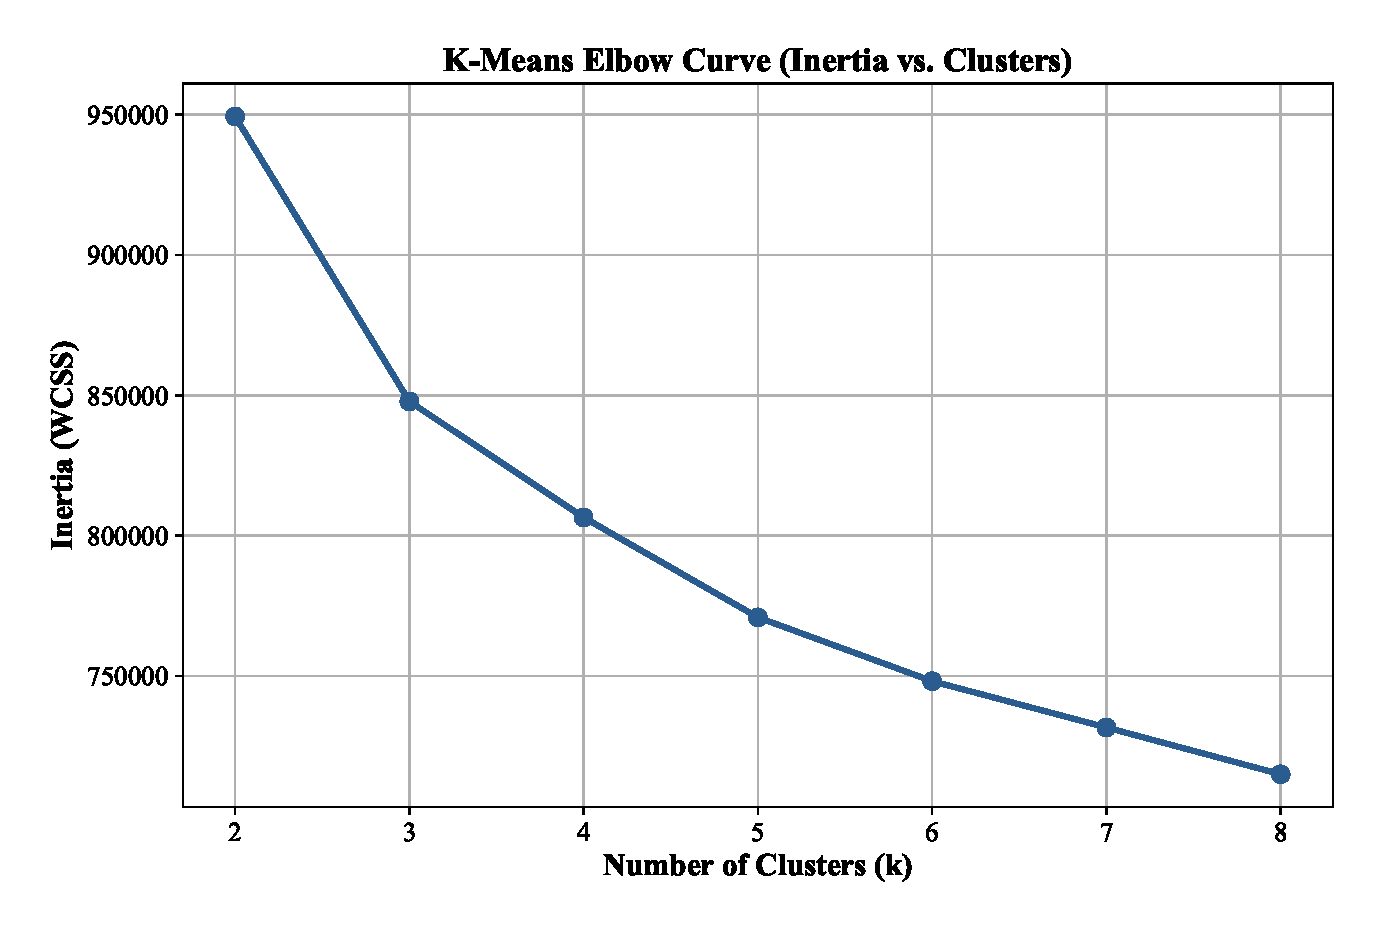
\includegraphics[width=\linewidth]{Elbow_Curve.eps}
    \caption{K-Means Elbow Curve (Inertia vs. $k$).}
    \label{fig:elbow}
\end{minipage}\hfill
\begin{minipage}{0.48\textwidth}
    \centering
    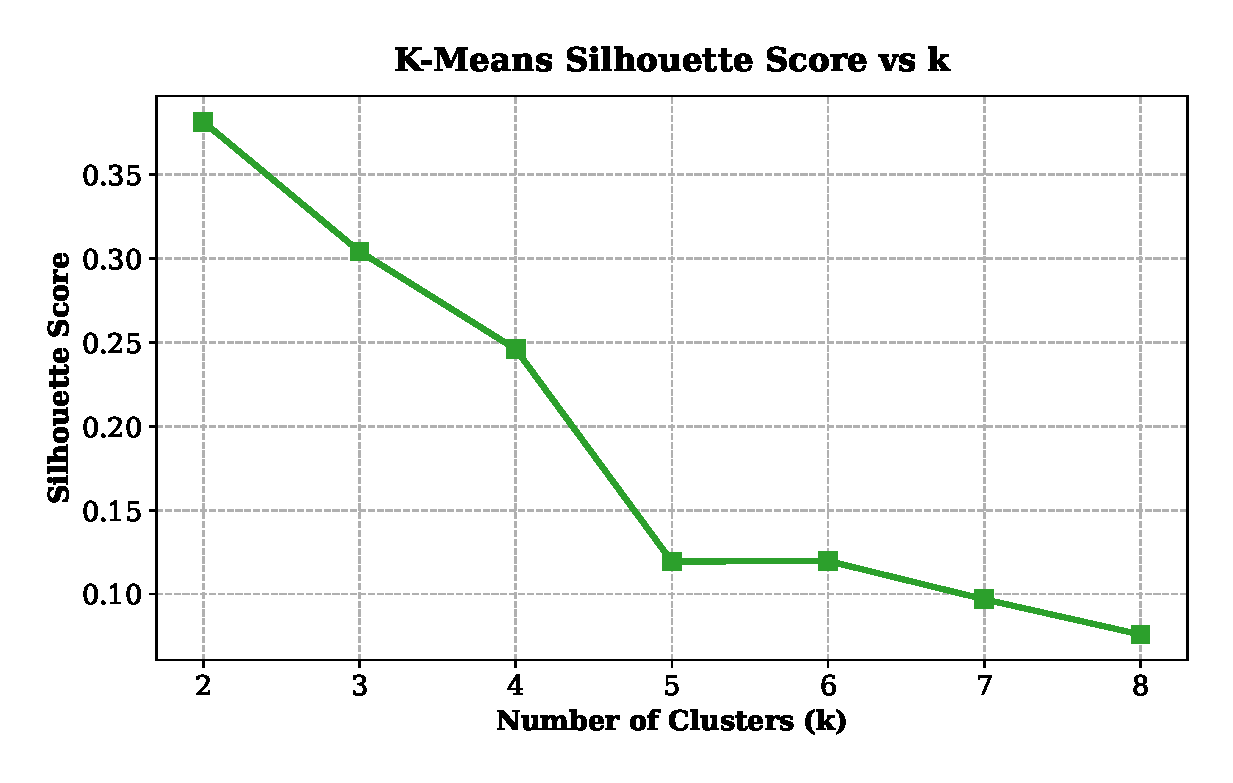
\includegraphics[width=\linewidth]{Silhouette_Curve.eps}
    \caption{Silhouette Score vs. Cluster Count $k$.}
    \label{fig:sil}
\end{minipage}
\end{figure}

\textbf{Inference (Elbow and Silhouette Curves):}
The Elbow curve displays a visible reduction in the rate of inertia drop after $k=2$ and $k=6$. The Silhouette score peaks at $k=2$ ($0.3815$) representing the dominant distinction between active movement and stillness, while stabilizing at $k=6$ ($0.1198$), justifying $k=6$ as the operational cluster partition.

\begin{figure}[H]
\centering
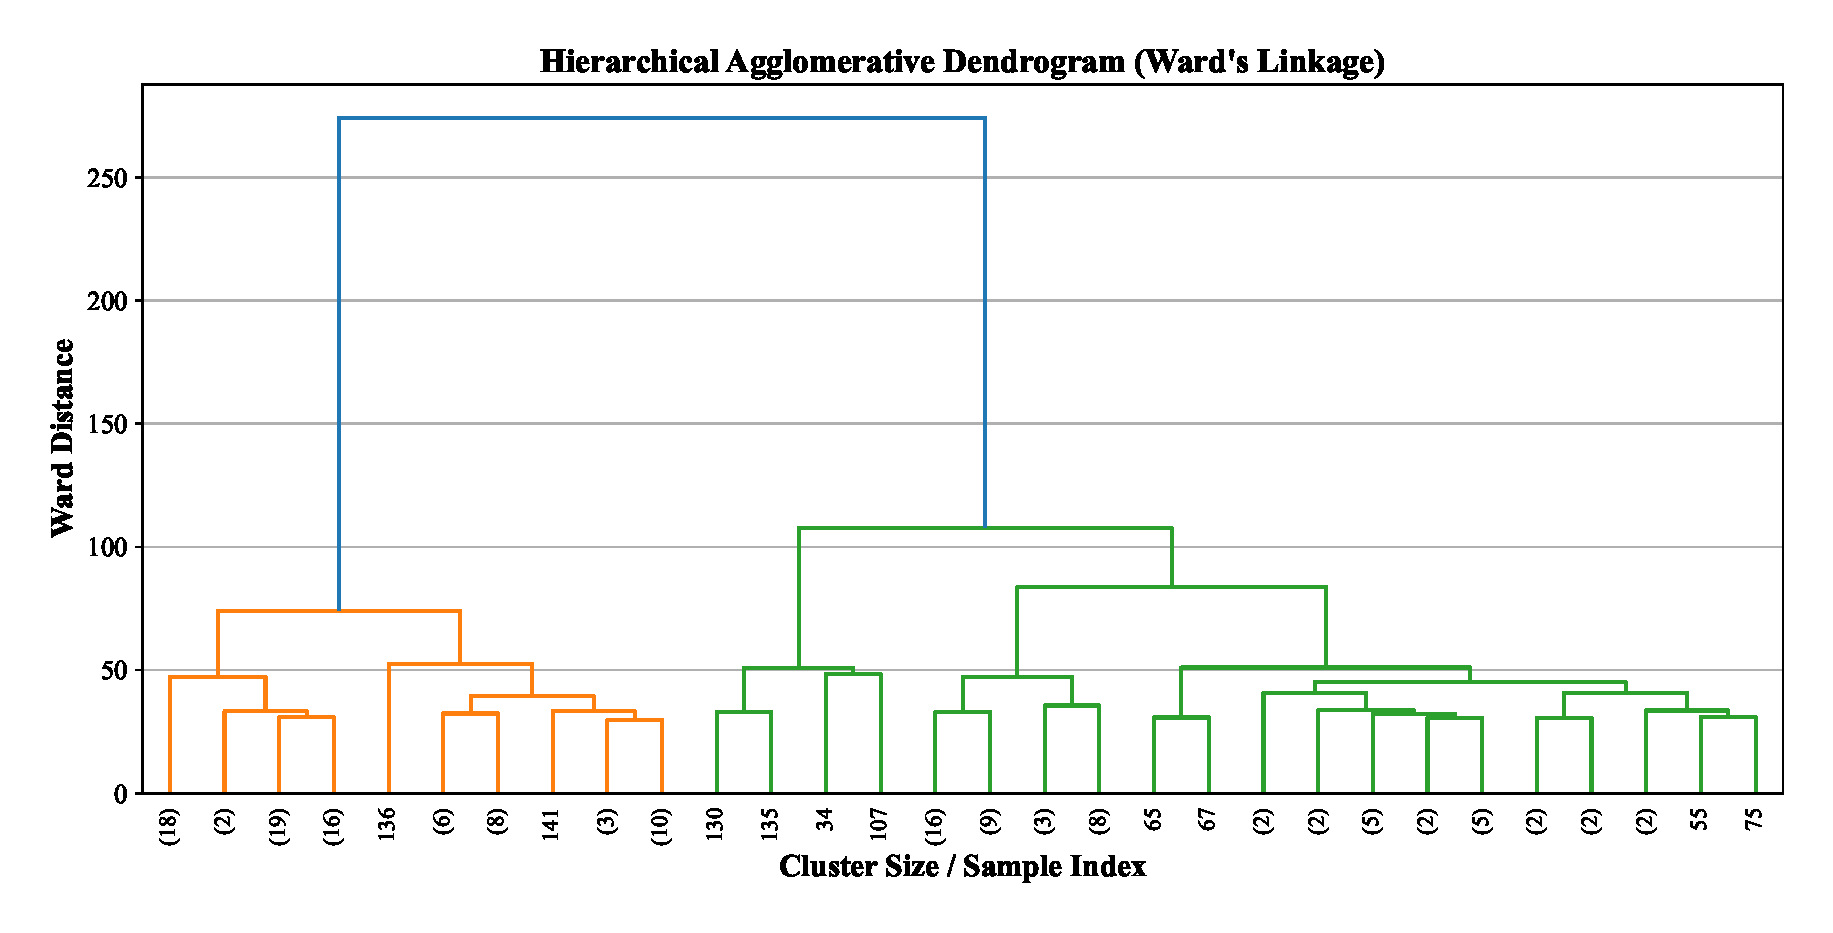
\includegraphics[width=0.88\linewidth]{Dendrogram.eps}
\caption{Hierarchical Agglomerative Dendrogram (Ward's Linkage).}
\label{fig:dendro}
\end{figure}

\textbf{Inference:}
The dendrogram reveals two major branches at the top hierarchy corresponding exactly to dynamic kinetic activities versus static postures. The subsequent subordinate splits progressively resolve walking variations and sitting/standing postures.

\begin{figure}[H]
\centering
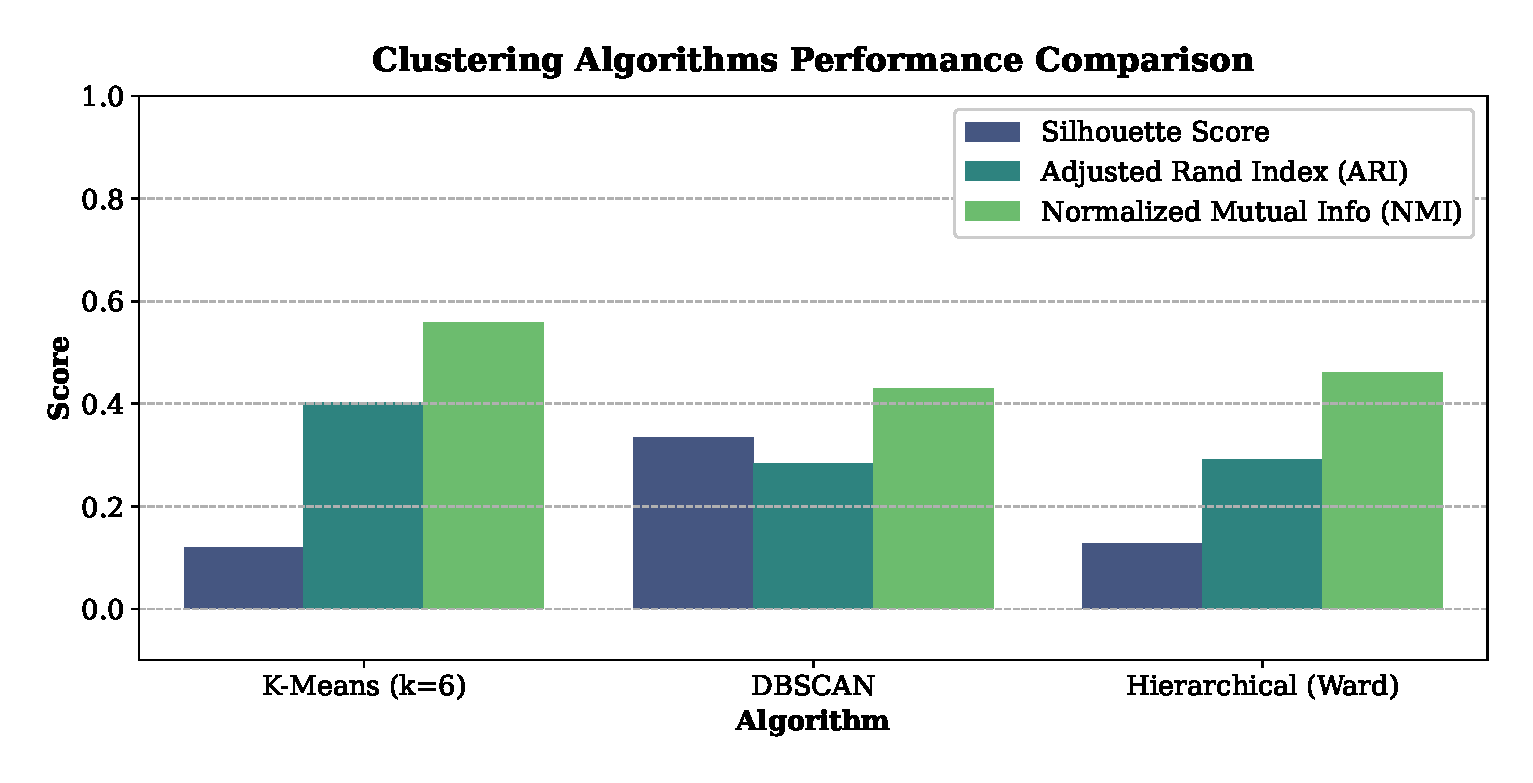
\includegraphics[width=0.85\linewidth]{Clustering_Comparison.eps}
\caption{Clustering Quality Validation Comparison Across Algorithms.}
\label{fig:comp_bar}
\end{figure}

\textbf{Inference:}
K-Means achieves the highest external label concordance ($\text{ARI} = 0.4034$, $\text{NMI} = 0.5582$), demonstrating that inertial features are well-approximated by centroid-based spherical partitioning. DBSCAN scores higher on density-based internal silhouette but groups overlapping postural classes into a unified density cluster.

\section{Discussion}
\subsection{Answers to Faculty Observation Questions}
\begin{enumerate}
    \item \textbf{Which algorithm produced the most meaningful clusters? Why?} \\
    \textbf{K-Means ($k=6$)} produced the most meaningful clusters, obtaining the highest external ground-truth metrics ($\text{ARI} = 0.4034$, $\text{NMI} = 0.5582$, and $\text{Calinski-Harabasz} = 741.37$). It successfully resolved cyclic accelerations into distinct walking subclasses.
    \item \textbf{How sensitive was K-Means to the choice of $k$?} \\
    Highly sensitive. At $k=2$, Silhouette peaks ($0.3815$) by splitting dynamic movements from postures. Increasing $k$ to 6 lowers WCSS by 22\%, but forces boundaries across overlapping postural densities.
    \item \textbf{Did DBSCAN detect noise or small clusters effectively?} \\
    Yes. In 561-dimensional sensor space, Euclidean distances concentrate. At $\epsilon=15.0, minPts=15$, DBSCAN effectively filtered transition outliers (34.57\% noise) while capturing dense steady-state movement cores.
    \item \textbf{How does linkage choice affect hierarchical clustering?} \\
    Ward's linkage was optimal ($\text{CH} = 705.32, \text{ARI} = 0.2913$) by minimizing variance inflation. In contrast, Single linkage suffered from severe chaining, merging outliers into an uninformative single cluster.
    \item \textbf{Which internal metric best matched visual intuition?} \\
    The \textbf{Calinski-Harabasz Index} and \textbf{Davies-Bouldin Index} best matched visual cluster compactivity on 2D projections, accurately favoring compact, distinct kinetic spheres over irregular density bands.
\end{enumerate}

\section{Conclusion}
Experiment 8 demonstrated unsupervised pattern discovery on complex human activity sensor streams. K-Means ($k=6$) and Ward's HAC successfully grouped physical activities aligning with ground-truth kinematics, while DBSCAN provided robust noise filtering against body transition artifacts.

\section*{References}
\begin{enumerate}[noitemsep]
    \item D. Anguita et al., ``A public domain dataset for human activity recognition using smartphones,'' \textit{ESANN}, 2013.
    \item P. J. Rousseeuw, ``Silhouettes: a graphical aid to the interpretation and validation of cluster analysis,'' \textit{J. Comput. Appl. Math.}, vol. 20, pp. 53--65, 1987.
    \item M. Ester et al., ``A density-based algorithm for discovering clusters in large spatial databases with noise,'' \textit{KDD}, vol. 96, pp. 226--231, 1996.
\end{enumerate}

\end{document}

